% !TEX root = tracking.tex
\section{General Framework \label{sec:framework}}
The overall framework of FaSTrackHD is summarized in Figs. \ref{fig:fw_online}, \ref{fig:hybrid_ctrl}, \ref{fig:fw_offline}. The online real-time framework is shown in Fig. \ref{fig:fw_online}. At the center of this framework is the path or trajectory planner; our framework is agnostic to the planner, so any may be used (e.g. MPC, RRT, neural networks). We will present an example using an RRT planner in Section \ref{sec:results}.
\begin{figure}[h!]
  \centering
	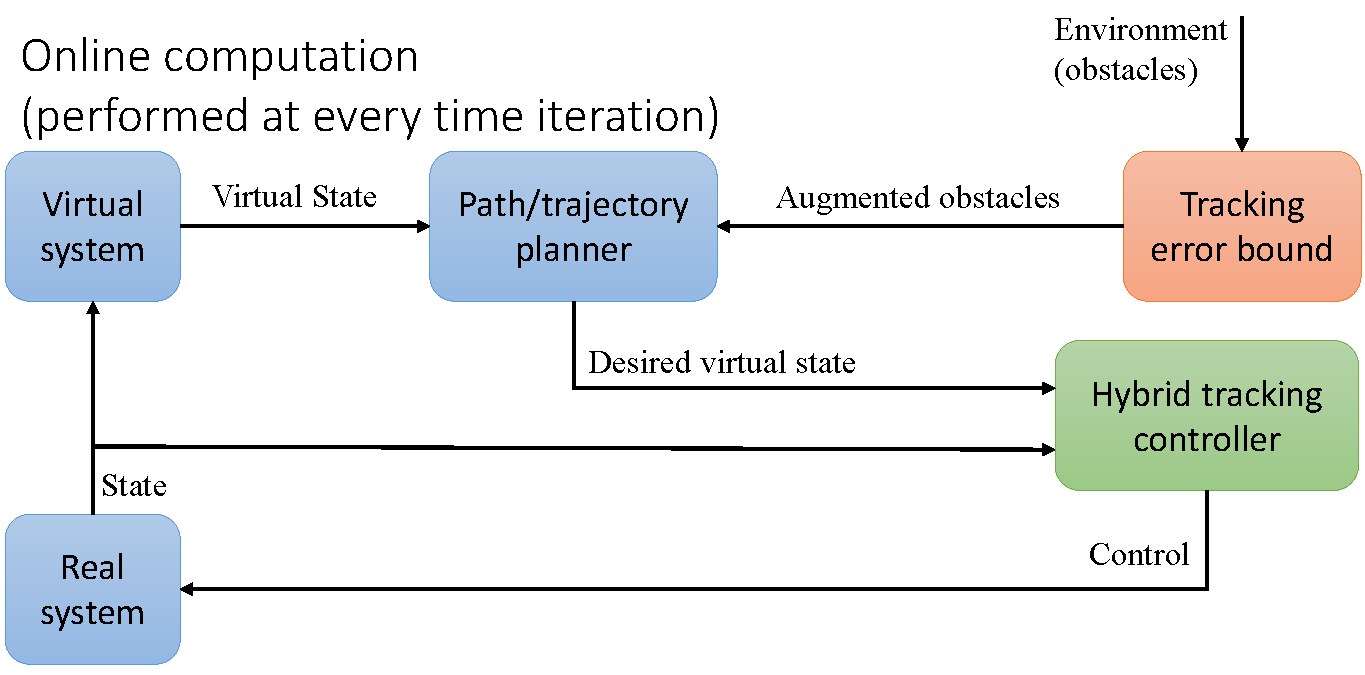
\includegraphics[width=1\columnwidth]{fig/framework_online}
	\caption{Online framework}
	\label{fig:fw_online}
	\vspace{-.1in}
\end{figure}

When executing the online framework, the first step is to sense obstacles in the environment, and then augment the sensed obstacles by a precomputed tracking error bound as described in Section \ref{sec:precomp}. This tracking error bound is a safety margin that guarantees robustness despite the worst-case disturbance. Augmenting the obstacles by this margin can be thought of as equivalent to wrapping the planning system with a ``safety bubble". These augmented obstacles are given as inputs to the planner along with the current state of the planning system. The planner then outputs the next desired state of the planning system. 

The tracking system is a model of the physical system (such as a quadrotor). The hybrid tracking controller block takes in the state of the tracking system as well as the desired state of the planning system. Based on the relative state between these two systems, the hybrid tracking controller outputs a control signal to the tracking system. The goal of this control is to make the tracking system track the desired planning state as closely as possible.

%In the context of real-time robust planning towards a target in an unknown environment, we propose a framework for combining fast planning methods that do not need to take into account disturbances, and HJ reachability analysis which provides formal guarantees for systems with disturbances. The high level idea of the framework is summarized in Fig. \ref{fig:fw_online}, \ref{fig:hybrid_ctrl}, and \ref{fig:fw_offline}. Formal definitions will be introduced in \MCnote{Section \ref{}}.

%Fig. \ref{fig:fw_online} shows the online computations under our framework, which uses a hierarchical structure in which a planner plans a path or trajectory for a simple ``virtual system''. Examples of planners include those based on model-predictive control (MPC), rapidly-exploring random tree (RRT), or neural networks; our framework is agnostic to the planner, so any planner can be used. The choice of the virtual system is also flexible, and depends on the requirements of the planner. We will present an example of a virtual system used in conjunction with an RRT planner in \MCnote{Section \ref{}}. The planner outputs a desired ``virtual state'' of the virtual system.

%The ``real system'' is a model of a physical system such as a quadrotor, and a subset of the state variables forms the virtual state of the virtual system. The state of real system and the desired virtual state are inputs to a hybrid tracking controller. Based on these two inputs, the hybrid tracking controller outputs a control signal to the real system. The goal of this control is to make the real system track the desired virtual state as closely as possible. Our concept of tracking error will be defined in \MCnote{Section \ref{}}.

The hybrid tracking controller is expanded in Fig. \ref{fig:hybrid_ctrl} and consists of two controllers: a safety controller and a performance controller. In general, there may be multiple safety and performance controllers depending on various factors such as observed size of disturbances, but for simplicity we will just consider one safety and one performance controller in this paper. The safety controller consists of a function (or look-up table) computed offline via HJ reachability, and guarantees that the tracking error bound is not violated, \textit{despite the worst-case disturbance}. In addition, the table look-up operation is computationally inexpensive. When the system is close to violating the tracking error bound, the safety controller must be used to prevent the violation. On the other hand, when the system is far from violating the tracking error bound, any controller (such as one that minimizes fuel usage), can be used. This control is used to update the tracking system, which in turn updates the planning system, and the process repeats.
\begin{figure}[h!]
  \centering
	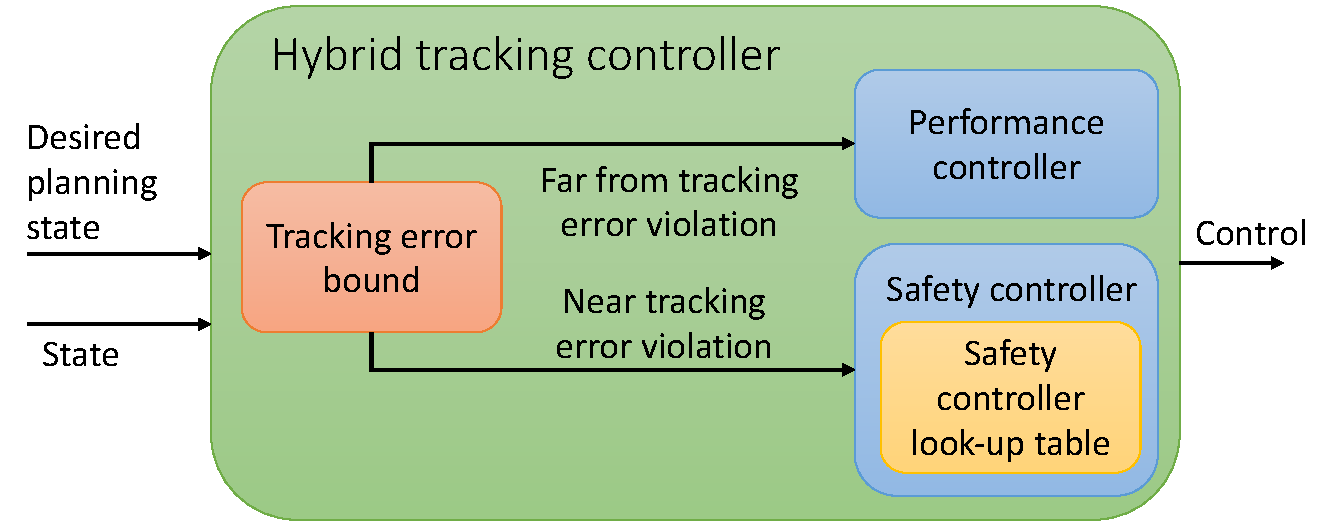
\includegraphics[width=0.9\columnwidth]{fig/hybrid_controller}
	\caption{Hybrid controller}
	\label{fig:hybrid_ctrl}
	\vspace{-.1in}
\end{figure}

To determine both the tracking error bound and safety controller functions/look-up tables, an offline framework is used as shown in Fig. \ref{fig:fw_offline}. The planning and tracking system dynamics are plugged into an HJ reachability computation, which computes a value function that acts as the tracking error bound function/look-up table. The spatial gradients of the value function comprise the safety controller function/look-up table. These functions are independent of the online computations---they depend only on the \textit{relative} states and dynamics between the planning and tracking systems, not on the absolute states along the trajectory at execution time.
\begin{figure}[h!]
  \centering
	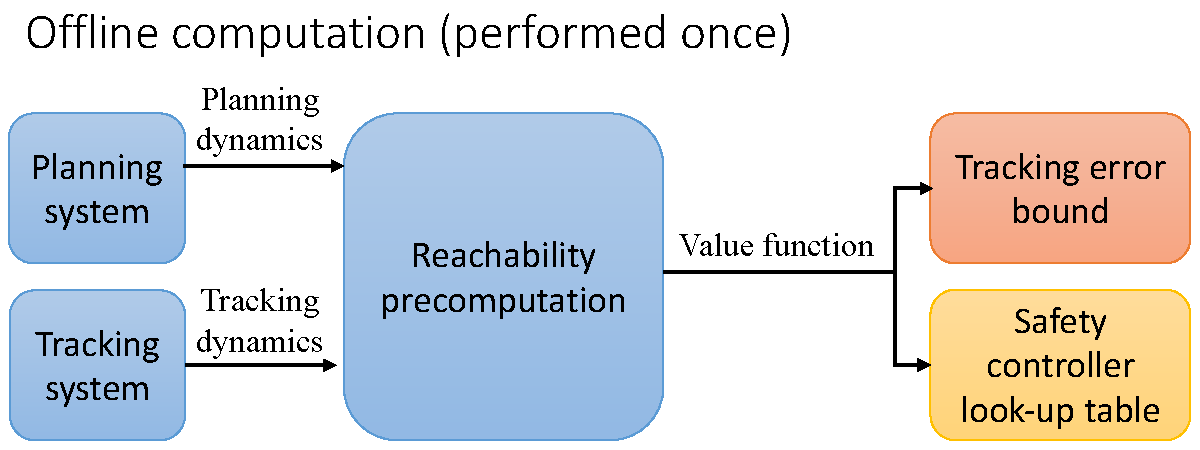
\includegraphics[width=0.9\columnwidth]{fig/framework_offline}
	\caption{Offline framework}
	\label{fig:fw_offline}
	%\vspace{-.1in}
\end{figure}

In the following sections we will first explain the precomputation steps taken in the offline framework. We will then walk through the online framework and provide a complete example.
%Besides the virtual state, the planner also takes into account any obstacles that must be avoided. In order to be robust to disturbances, planning must be done with a safety margin that accounts for disturbances. A safety margin that guarantees robustness despite the worst-case disturbance is given by a tracking error bound obtained in the offline HJ reachability computation, shown in Fig. \ref{fig:fw_offline} and explained in detail in \MCnote{Section \ref{}}. The virtual and real system dynamics are used to compute a value function, which simultaneously gives the tracking error bound and the safety controller look-up table used by the hybrid tracking controller.
%
%\textbf{Maybe put next paragraph in the introduction}
%
%There are many fast planners that could potentially do planning in real-time; however, these typically cannot account for disturbances in a provably safe way. In addition, complex system models with nonlinear dynamics complicate planning algorithms (non-convex for MPC, more difficult for RRT). On the other hand, HJ reachability is able to handle disturbances, and is agnostic to system dynamics. In addition, provably guarantees can be provided. However, HJ reachability and in general formal verification methods can be very expensive to compute.
%
%Refer to figure: planning level and safety level. 
%
%In the safety level, we start with the error dynamics, and we compute two things: bubble which is fed into planner to plan with extra margin, and error-feedback controller for real-time control. These two can be computed offline independent of the planned path.
%
%In the planning level, any planning method such as MPC, RRT, etc. (cite some things) can be used. The planning level does not need to take into account disturbances, and can use simple system dynamics or even no dynamics at all. In fact we will be using a simple RRT planner which simply provides paths, in the form of a sequence of line segments, which are not dynamically feasible. 
